\documentclass[11pt,a4paper]{article}
\usepackage[spanish,es-nodecimaldot]{babel}	% Utilizar español
\usepackage[utf8]{inputenc}					% Caracteres UTF-8
\usepackage{graphicx}						% Imagenes
\usepackage[hidelinks]{hyperref}			% Poner enlaces sin marcarlos en rojo
\usepackage{fancyhdr}						% Modificar encabezados y pies de pagina
\usepackage{float}							% Insertar figuras
\usepackage[textwidth=390pt]{geometry}		% Anchura de la pagina
\usepackage[nottoc]{tocbibind}				% Referencias (no incluir num pagina indice en Indice)
\usepackage{enumitem}						% Permitir enumerate con distintos simbolos
\usepackage[T1]{fontenc}					% Usar textsc en sections
\usepackage{amsmath}						% Símbolos matemáticos

\usepackage{listings}
\usepackage[dvipsnames]{xcolor}

\definecolor{codegreen}{rgb}{0,0.6,0}
\definecolor{codegray}{rgb}{0.5,0.5,0.5}
\definecolor{codepurple}{rgb}{0.58,0,0.82}
\definecolor{backcolour}{rgb}{0.95,0.95,0.92}

\lstdefinestyle{mystyle}{
    backgroundcolor=\color{backcolour},   
    commentstyle=\color{codegreen},
    keywordstyle=\color{magenta},
    numberstyle=\tiny\color{codegray},
    stringstyle=\color{codepurple},
    basicstyle=\ttfamily\footnotesize,
    breakatwhitespace=false,         
    breaklines=true,                 
    captionpos=b,                    
    keepspaces=true,                 
    numbers=left,                    
    numbersep=5pt,                  
    showspaces=false,                
    showstringspaces=false,
    showtabs=false,                  
    tabsize=4,
    language=C++
}

\usepackage{fancyvrb}

% redefine \VerbatimInput
\RecustomVerbatimCommand{\VerbatimInput}{VerbatimInput}%
{fontsize=\footnotesize,
 %
 commandchars=\|\(\), % escape character and argument delimiters for
                      % commands within the verbatim
 commentchar=*        % comment character
}

\lstset{style=mystyle}

% Comando para poner el nombre de la asignatura
\newcommand{\asignatura}{Arquitectura y Computación de Altas Prestaciones}
\newcommand{\autor}{Vladislav Nikolov Vasilev}
\newcommand{\titulo}{Práctica 5}
\newcommand{\subtitulo}{Suma de vectores con CUDA}
\newcommand{\rama}{Ingeniería de Computadores}

% Comando vector
\renewcommand{\vec}[1]{\mathbf{#1}}

% Configuracion de encabezados y pies de pagina
\pagestyle{fancy}
\lhead{\autor{}}
\rhead{\asignatura{}}
\lfoot{Grado en Ingeniería Informática}
\cfoot{}
\rfoot{\thepage}
\renewcommand{\headrulewidth}{0.4pt}		% Linea cabeza de pagina
\renewcommand{\footrulewidth}{0.4pt}		% Linea pie de pagina

\begin{document}
\pagenumbering{gobble}

% Pagina de titulo
\begin{titlepage}

\begin{minipage}{\textwidth}

\centering

%
\includegraphics[scale=0.5]{img/ugr.png}\\

\includegraphics[scale=0.3]{img/logo_ugr.jpg}\\[1cm]

\textsc{\Large \asignatura{}\\[0.2cm]}
\textsc{GRADO EN INGENIERÍA INFORMÁTICA}\\[1cm]

\noindent\rule[-1ex]{\textwidth}{1pt}\\[1.5ex]
\textsc{{\Huge \titulo\\[0.5ex]}}
\textsc{{\Large \subtitulo\\}}
\noindent\rule[-1ex]{\textwidth}{2pt}\\[3.5ex]

\end{minipage}

%\vspace{0.5cm}
\vspace{0.7cm}

\begin{minipage}{\textwidth}

\centering

\textbf{Autor}\\ {\autor{}}\\[2.5ex]
\textbf{Rama}\\ {\rama}\\[2.5ex]
\vspace{0.3cm}


\includegraphics[scale=0.3]{img/etsiit.jpeg}

\vspace{0.7cm}
\textsc{Escuela Técnica Superior de Ingenierías Informática y de Telecomunicación}\\
\vspace{1cm}
\textsc{Curso 2019-2020}
\end{minipage}
\end{titlepage}

\pagenumbering{arabic}
\tableofcontents
\thispagestyle{empty}				% No usar estilo en la pagina de indice

\newpage

\setlength{\parskip}{1em}

\section{Introducción}

En esta práctica se pide implementar dos versiones de un mismo programa: una primera
versión secuencial y una versión en \texttt{CUDA}. El objetivo del programa es, dados
dos vectores $\vec{A}$ y $\vec{B}$, ambos de tamaño $n$, obtener un vector de salida
$\vec{C}$ del mismo tamaño en el que $\forall \vec{C}_i \in \vec{C}$, su valor
venga determinado por la expresión:

\begin{equation}
\vec{C}_i =
\Bigg(
\bigg(
\frac{\log(5 \cdot \vec{A}_i \cdot 100 \cdot \vec{B}_i) + 7 \cdot \vec{A}_i}{0.33}
\bigg)^3 \Bigg)^7
\label{eq:formula}
\end{equation}

Además, se ha especificado que los vectores de entrada $\vec{A}$ y $\vec{B}$
se tienen que replicar un número de veces, de forma que su longitud se vea incrementada.
En este caso, se ha decidido \textbf{que se van a tener 5 copias de los vectores originales},
es decir, que los vectores van a tener una longitud de $5n$, donde $n$ es el tamaño
original especificado en los archivos proporcionados.

Para cada uno de los nueve problemas proporcionados se van a tomar medidas
de tiempo de lo que se tarda en hacer todas las operaciones con los dos programas.
Con ellas se representará la evolución del tiempo de ejecución en cada caso en función
del tamaño del problema y se hará un estudio de la ganancia.

Adicionalmente, se pide que se obtengan las especificaciones de la \texttt{GPU} que se está
utilizando, de manera que se tenga más infomración sobre esta.

\section{Especificaciones de la \texttt{GPU}}

Primeramente vamos a ver cuáles son las especificaciones de la \texttt{GPU} que vamos a
utilizar. Para ello se ha creado un programa que puede encontrarse en el archivo
\texttt{deviceProperties.cu}, el cuál muestra la siguiente información:

\begin{itemize}
  \item Nombre del dispositivo.
  \item Número de SMs (procesadores).
  \item Número de SPs por SM (cores por procesador).
  \item Número total de SPs.
  \item Memoria total de la gráfica en MB.
  \item Memoria compartida por SM en KB.
  \item Memoria compartida por bloque en KB.
  \item Número máximo de hebras por bloque.
  \item Número máximo de hebras por cada dimensión.
\end{itemize}

El código que muestra esta información es el siguiente:

\begin{lstlisting}
int main()
{
    int n_devices;

    cudaGetDeviceCount(&n_devices);

    int i;

    for (i = 0; i < n_devices; i++)
    {
        cudaDeviceProp prop;
        cudaGetDeviceProperties(&prop, i);
        int numSPs = getSPcores(prop);

        printf("Device number: %d\n", i);
        printf(" Device name: %s\n", prop.name);
        printf(" Number of SMs: %d\n", prop.multiProcessorCount);
        printf(" Number of SPs per SM: %d\n", numSPs);
        printf(" Total Number of SPs: %d\n", numSPs * prop.multiProcessorCount);
        printf(" Total Available Global Memory Size (MB): %zu\n", prop.totalGlobalMem / (1<<20));
        printf(" Shared Memory Per SM (KB): %zu\n", prop.sharedMemPerMultiprocessor / (1<<10));
        printf(" Shared Memory Per Block (KB): %zu\n", prop.sharedMemPerBlock / (1<<10));
        printf(" Max. Threads Per Block: %d\n", prop.maxThreadsPerBlock);
        printf(" Max. Threads Per Dimension: x: %d, y: %d, z: %d\n",
                prop.maxThreadsDim[0], prop.maxThreadsDim[1], prop.maxThreadsDim[2]);
    }

    return 0;
}
\end{lstlisting}

La función \texttt{getSPcores} se ha extraído de una respuesta a una pregunta en
\textit{StackOverflow} \cite{cuda-sp}. En caso de tener más de una tarjeta gráfica
(que no es el caso), se mostraría la información para cada una de ellas. En este
caso se ha obtenido la siguiente información:

\VerbatimInput{../out/specs.txt}

\section{Versión secuencial}

Una vez que hemos visto las especificaciones de nuestra gráfica, vamos a ver cómo sería
una primera versión secuencial del programa.

La versión secuencial carga los ficheros de datos que se han especificado como parámetros,
carga los valores, los copia un número de veces que se determina como parámetro y realiza
la operación, obteniendo el vector $\vec{C}$ de salida. La función que realiza el cálculo
que se puede ver en la ecuación \eqref{eq:formula} es la siguiente:

\begin{lstlisting}
void add_vectors(float *A, float *B, float *C, int N)
{
    int i;

    for (i = 0; i < N; i++)
    {
        C[i] = pow(pow(log(5*A[i]*100*B[i] + 7*A[i]) / 0.33, 3), 7);
    }
}
\end{lstlisting}

La función recibe como parámetro los dos vectores de entrada, el de salida y el
tamaño de los vectores, y con un bucle recorre los elementos de $\vec{A}$ y $\vec{B}$
y calcula el correspondiente elemento de $\vec{C}$.

El resto del código se encuentra en el archivo \texttt{vectorAdd.c} y se puede consultar
de ser necesario. Como en general son operaciones sencillas, no se van a explicar ni a incluir
aquí, ya que no se considera que estén relacionadas con la asignatura (lectura de ficheros,
reserva de memoria, etc.).

\section{Versión paralela con \texttt{CUDA}}

Una vez implementada y probada la versión secuencial se ha procedido a desarrollar
la versión paralela.

\section{Resultados}

\begin{figure}[H]
  \centering
  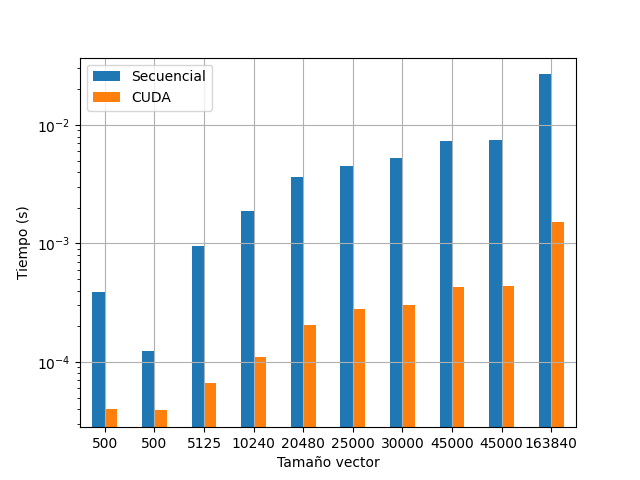
\includegraphics[scale=0.6]{img/seq-cuda}
  \caption{Evolución del tiempo de ejecución del programa secuencial y el programa en
  \texttt{CUDA} en función del tamaño del vector con escala logarítmica en el eje $Y$.}
  \label{fig:seq-cuda}
\end{figure}

\begin{figure}[H]
  \centering
  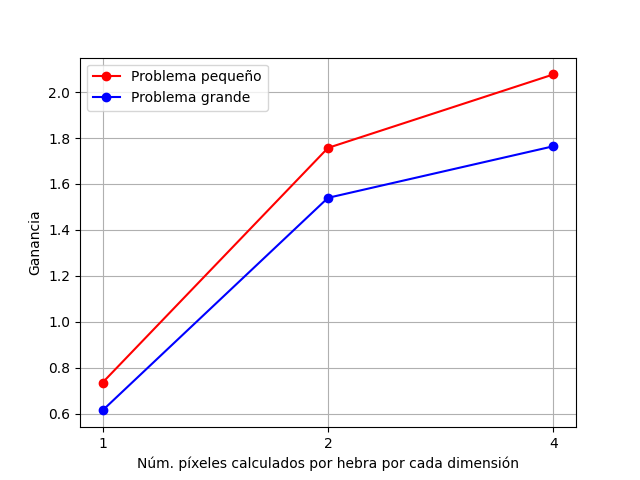
\includegraphics[scale=0.6]{img/speedup}
  \caption{Ganancia obtenida en función del tamaño del vector.}
\end{figure}

\section{Conclusiones}

\newpage

\begin{thebibliography}{5}

\bibitem{cuda-sp}
StackOverflow. \textit{How can I get number of Cores in cuda device?}
\\\url{https://stackoverflow.com/questions/32530604/how-can-i-get-number-of-cores-in-cuda-device}

\end{thebibliography}

\end{document}

